% !TEX root = ../../lectures.tex
\section{Alfv\'en waves through a mechanical analogy}

Consider a uniform, perfectly conducting plasma at rest with a uniform magnetic field
\(\mathbf B_0\).
In ideal MHD the field is \emph{frozen} into the fluid, so a small sideways nudge of a fluid element relative to \(\mathbf B_0\) bends the field lines. Bending stores magnetic energy, and the field responds with a \emph{tension} that tries to straighten the lines. This tension provides the restoring force that launches a disturbance along \(\mathbf B_0\).

It is convenient to write the magnetic force per unit volume (the magnetic force density) as
\[
\mathbf f
= \frac{1}{4\pi}(\mathbf B\!\cdot\!\nabla)\mathbf B
\;-\;\nabla\!\left(\frac{B^2}{8\pi}\right).
\]

The second term acts like an isotropic \emph{magnetic pressure}; the first is the \emph{magnetic tension} that pulls along the field direction. If a field line is bent with radius of curvature \(R\), the tension generates a transverse restoring force of order
\[
f_\perp \sim \frac{B_0^2}{4\pi}\,\frac{1}{R},
\]
precisely the behavior of a taut string that resists curvature!

To make this analogy quantitative, take a thin magnetic \emph{flux tube} of cross-section \(A\) following \(\mathbf B_0\), and let \(s\) be arc length along the unperturbed field. A small transverse displacement \(\xi_\perp(s,t)\) introduces curvature \(\kappa \approx \partial_s^2 \xi_\perp\).
The tension acting on a short segment of length \(\Delta s\) is then
\[
F_\perp \;=\; \Big(\frac{B_0^2}{4\pi}\Big) A\,\frac{\partial^2 \xi_\perp}{\partial s^2}\,\Delta s,
\]
because the field exerts a tension \(B_0^2/4\pi\) per unit area along the tube.
The segment’s mass is \(\rho\,A\,\Delta s\), so Newton’s second law gives
\[
\rho A\,\Delta s\,\frac{\partial^2\xi_\perp}{\partial t^2}
\;=\;
\Big(\frac{B_0^2}{4\pi}\Big) A\,\frac{\partial^2 \xi_\perp}{\partial s^2}\,\Delta s.
\]
Canceling \(A\Delta s\) yields the transverse wave equation
\[
\frac{\partial^2\xi_\perp}{\partial t^2}
\;=\;
\frac{B_0^2}{4\pi\rho}\,\frac{\partial^2\xi_\perp}{\partial s^2}.
\]

At this point the identification with the vibrating string is immediate. The string equation
\(\partial_t^2 \xi = (T/\mu)\,\partial_s^2 \xi\)
involves a \emph{tension} \(T\) and a \emph{linear mass density} \(\mu\).
For our flux tube,
\[
T=\frac{B_0^2}{4\pi}\,A,
\quad \text{and} \quad
\mu=\rho\,A,
\]
so that \(T/\mu = B_0^2/(4\pi\rho)\).
The solution of the string equation is given in terms of a wave with speed
\begin{remark}
\[
v_A \;=\; \sqrt{\tfrac{T}{\mu}} \;=\; \frac{B_0}{\sqrt{4\pi\rho}}
\]
\end{remark}
%Notice how the cross-section \(A\) cancels: only \(B_0\) and \(\rho\) matter.

\begin{figure}[t] 
\centering 
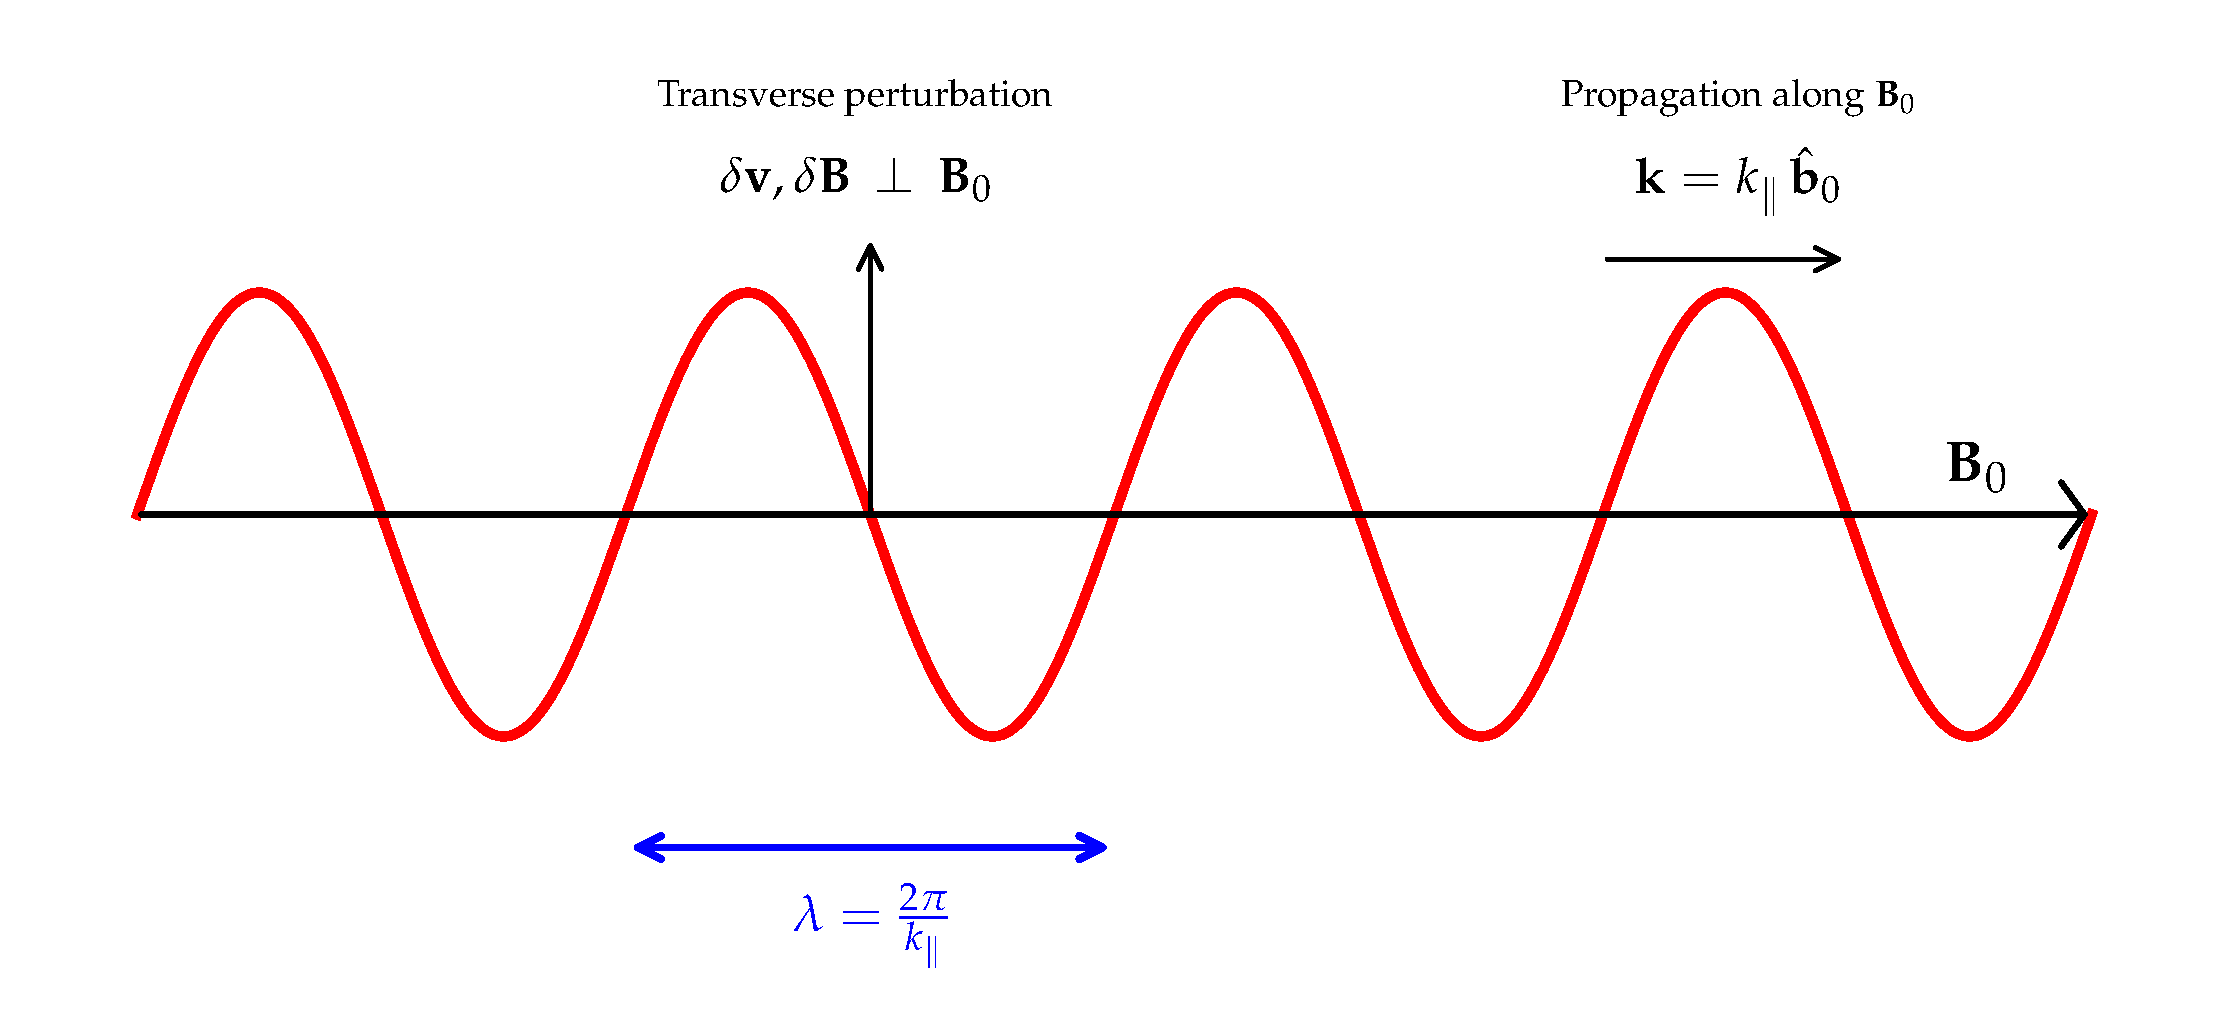
\includegraphics[width=\textwidth]{figures/alfven_diagram.pdf}
\caption{.} 
\label{fig:alfvenwave} 
\end{figure}

Why does an Alfvén disturbance propagate \emph{along} \(\mathbf B_0\)?
Because the restoring force is magnetic \emph{tension}—it arises from field-line curvature, which requires variation \emph{along} the field. If the wavevector has no component along \(\mathbf B_0\) (\(k_\parallel=0\)), the field lines are not bent and the tension vanishes to leading order: there is no shear-Alfvén propagation. In the linear regime this is reflected by the dispersion relation
\[
\omega=\pm k_\parallel v_A,
\]
which depends only on the parallel component of the wavevector.

Energetically, the picture mirrors the lossless string: as the wave oscillates, magnetic bending energy converts into kinetic energy and back again, with equal time-averaged contributions. The magnetic-pressure term is unchanged to leading order for a pure Alfvén mode; it is the tension piece that does the “work”.

\begin{remark}{Characteristic speeds in ISM}

For the Alfv\'en speed in the ISM we use
\[
v_A \simeq \frac{B}{\sqrt{4\pi\,\rho}}
\;\approx\;
\frac{B}{\sqrt{4\pi\,m_p\,n_i}},
\]
where \(n_i\) is the ion number density.  
In the warm ISM, taking \(B \sim 5~\mu\mathrm{G}\) and \(n_i \sim 1~\mathrm{cm^{-3}}\) gives
\[
v_A \sim 10\text{--}20~\mathrm{km\,s^{-1}}.
\]
This is tiny compared with relativistic particle speeds, so cosmic rays (with \(v\simeq c\)) effectively \emph{see} Alfv\'en waves as stationary scattering centers in many Galactic environments.

For comparison, the adiabatic sound speed
%\[
%c_s=\sqrt{\frac{\gamma k_B T}{\mu m_p}}
%\]
is \(c_s \approx 10~\mathrm{km\,s^{-1}}\) for a typical warm ISM temperature \(T\!\sim\!8000~\mathrm{K}\) (with reasonable \(\mu\) and \(\gamma\)). Thus Alfv\'en and sound speeds are of the same order, implying a plasma beta
\[
\beta \equiv \frac{8\pi p}{B^2} \sim \mathcal O (1)
\]
near unity in these phases.

In the \emph{solar corona}, the parameters are very different: \(B_0\!\sim\!10~\mathrm{G}\) and \(n\!\sim\!10^9~\mathrm{cm^{-3}}\) yield
\( 
v_A \approx 690~\mathrm{km\,s^{-1}},
\)
typically much larger than \(c_s\) there, i.e.\ \(\beta \ll 1\). In short: the warm ISM is a \(\beta\!\sim\!1\) environment with \(v_A\!\sim\!c_s\), whereas the corona is tension-dominated with \(v_A\!\gg\!c_s\).
\end{remark}

%\subsection{Alfv\'en Waves (vs.\ Sound Waves)}
%
%\paragraph{Setting and assumptions.}
%We work in (ideal) MHD with a uniform equilibrium:
%\[
%\mathbf{B}_0=\text{const},\qquad \rho_0=\text{const},\qquad \mathbf{v}_0=\mathbf{0},\qquad p_0=\text{const}.
%\]
%Small perturbations $\delta \rho,\,\delta p,\,\delta \mathbf{v},\,\delta \mathbf{B}$ vary as $\exp[i(\mathbf{k}\!\cdot\!\mathbf{x}-\omega t)]$.
%The ideal MHD equations we linearize are
%\[
%\begin{aligned}
%&\partial_t \rho + \nabla\!\cdot(\rho \mathbf{v}) = 0,\\
%&\rho\,\partial_t \mathbf{v} = -\nabla p + \frac{1}{\mu_0}(\nabla\times \mathbf{B})\times \mathbf{B},\\
%&\partial_t \mathbf{B} = \nabla\times(\mathbf{v}\times \mathbf{B}),\qquad \nabla\!\cdot\!\mathbf{B}=0,\\
%&\delta p = c_s^2\,\delta \rho\quad(\text{adiabatic closure, }c_s^2=\gamma p_0/\rho_0).
%\end{aligned}
%\]
%
%\paragraph{Alfv\'en waves: definition and dispersion.}
%Alfv\'en waves are \emph{transverse, incompressible} MHD waves whose restoring force is the magnetic tension of the background field $\mathbf{B}_0$.
%They satisfy
%\[
%\delta \rho = 0,\qquad \delta p = 0,\qquad \mathbf{k}\cdot \delta\mathbf{v}=0,
%\]
%with polarization $\delta\mathbf{v}\perp\mathbf{B}_0$ and $\delta\mathbf{B}\perp\mathbf{B}_0$.
%Writing $\mathbf{k}=k_\parallel \hat{\mathbf{b}}_0 + \mathbf{k}_\perp$ with $\hat{\mathbf{b}}_0=\mathbf{B}_0/B_0$, the dispersion relation is
%\[
%\boxed{\ \omega = \pm k_\parallel v_A\ ,\qquad v_A=\frac{B_0}{\sqrt{\mu_0 \rho_0}}\ } \quad
%\text{(SI)}\qquad\text{or}\qquad v_A=\frac{B_0}{\sqrt{4\pi \rho_0}}\ \text{(cgs)}.
%\]
%Key features:
%\begin{itemize}
%\item Propagate \emph{along field lines}: no propagation if $k_\parallel=0$.
%\item \emph{Transverse} polarization: $\delta\mathbf{v}\perp \mathbf{k}$ and $\delta\mathbf{v}\perp \mathbf{B}_0$ (shear Alfv\'en mode).
%\item \emph{Incompressible}: no density/pressure perturbations at leading order.
%\item Energy equipartition in linear waves: kinetic and magnetic perturbation energies are equal on average.
%\item Group and phase velocities are $\pm v_A\,\hat{\mathbf{b}}_0$ (purely along $\mathbf{B}_0$).
%\end{itemize}
%
%\paragraph{Physical picture.}
%Imagine a taut magnetic ``string'' (field line). A sideways displacement bends it, creating curvature and a \emph{tension} force $\propto B_0^2$ that pulls the plasma back; inertia is provided by $\rho_0$. The wave speed therefore scales as $v_A\propto B_0/\sqrt{\rho_0}$.
%
%\paragraph{Sound waves: contrast.}
%Ordinary sound waves in a neutral or weakly magnetized fluid have
%\[
%\boxed{\ \omega = \pm k\,c_s\ ,\qquad \delta\mathbf{v}\parallel \mathbf{k}\ ,\qquad \text{compressive}~(\delta\rho,\delta p\neq 0)\ }.
%\]
%They are longitudinal, isotropic (no preferred direction), and the restoring force is the \emph{gas pressure gradient}, not magnetic tension.
%
%\paragraph{Magnetized plasma taxonomy (for context).}
%In a magnetized plasma there are three linear MHD modes:
%\begin{enumerate}
%\item \textbf{Alfv\'en} (transverse, incompressible, $\omega=\pm k_\parallel v_A$).
%\item \textbf{Slow magnetosonic} (compressive, generally sub-$\min\{c_s,v_A\}$, strongly field-aligned at low $\beta$).
%\item \textbf{Fast magnetosonic} (compressive, more isotropic, super-$\max\{c_s,v_A\}$ at low $\beta$).
%\end{enumerate}
%The relative importance of these modes depends on the plasma beta
%\[
%\beta \equiv \frac{2\mu_0 p_0}{B_0^2} \quad \text{(SI)}\qquad \Big(\text{or } \beta=8\pi p_0/B_0^2\ \text{in cgs}\Big).
%\]
%Low-$\beta$ plasmas ($\beta\ll1$) are tension-dominated ($v_A\gg c_s$); high-$\beta$ plasmas behave more like ordinary fluids ($c_s\gtrsim v_A$).
%
%\paragraph{Polarization and correlations.}
%For linear Alfv\'en waves,
%\[
%\delta\mathbf{B} = \pm \sqrt{\mu_0 \rho_0}\,\delta\mathbf{v}\times \hat{\mathbf{b}}_0,\qquad
%\delta\mathbf{E} = -\,\delta\mathbf{v}\times \mathbf{B}_0,
%\]
%and the Poynting flux $\mathbf{S}=\mu_0^{-1}\,\delta\mathbf{E}\times \delta\mathbf{B}$ points along $\pm\hat{\mathbf{b}}_0$.
%
%\paragraph{Damping (very brief).}
%Ideal MHD is dissipationless. In real plasmas, Alfv\'en waves can damp via:
%viscosity/resistivity (Ohmic), ion–neutral friction (partially ionized media), phase mixing and resonant absorption (inhomogeneous $v_A$), and at smaller scales via kinetic effects (e.g.\ Landau/cyclotron damping; ``kinetic Alfv\'en'' regime when $k_\perp \rho_i\!\sim\!1$).
%%
%\paragraph{Worked numbers.}
%\begin{itemize}
%\item \emph{Warm ISM:} $B_0\!\sim\!5~\mu\text{G}$, $n\!\sim\!1~\text{cm}^{-3}$ $\Rightarrow$ 
%$v_A \approx 2.18\,\frac{B_{[\mu\text{G}]}}{\sqrt{n_{[\text{cm}^{-3}]}}}\,\text{km s}^{-1} \approx 11~\text{km s}^{-1}$.
%For $T\!\sim\!8000$ K, $c_s\!\approx\!9~\text{km s}^{-1}$, so Alfv\'en and sound speeds are comparable.
%\item \emph{Solar corona:} $B_0\!\sim\!10~\text{G}$, $n\!\sim\!10^9~\text{cm}^{-3}$ $\Rightarrow$
%$v_A \approx 2.18\,\frac{10^7}{\sqrt{10^9}} \approx 690~\text{km s}^{-1}$, typically $\gg c_s$ ($\beta\ll1$).
%\end{itemize}
%
%\paragraph{At-a-glance comparison.}
%\begin{center}
%\begin{tabular}{lcc}
%\toprule
% & \textbf{Alfv\'en wave} & \textbf{Sound wave} \\
%\midrule
%Restoring force & Magnetic tension ($\propto B_0^2$) & Gas pressure gradient \\
%Compressibility & Incompressible ($\delta \rho=0$) & Compressive ($\delta \rho\neq 0$) \\
%Polarization & Transverse ($\delta\mathbf{v}\perp \mathbf{k},\mathbf{B}_0$) & Longitudinal ($\delta\mathbf{v}\parallel \mathbf{k}$) \\
%Dispersion & $\omega=\pm k_\parallel v_A$ & $\omega=\pm k\,c_s$ \\
%Anisotropy & Propagates along $\mathbf{B}_0$ & Isotropic \\
%Energy flux & Along field lines & Along $\mathbf{k}$ \\
%Key parameter & $v_A=B_0/\sqrt{\mu_0\rho_0}$ & $c_s=\sqrt{\gamma p_0/\rho_0}$ \\
%\bottomrule
%\end{tabular}
%\end{center}
%
%\paragraph{Derivation sketch.}
%Taking $\mathbf{k}$ in the $x$–$z$ plane with $\mathbf{B}_0=B_0\hat{\mathbf{z}}$ and seeking a transverse solution with $\delta v_y\neq 0$, the linearized momentum and induction equations give
%\[
%-i\omega \rho_0\,\delta v_y = \frac{i k_\parallel B_0}{\mu_0}\,\delta B_y,\qquad
%-i\omega\,\delta B_y = i k_\parallel B_0\,\delta v_y,
%\]
%which combine to yield $\omega^2 = k_\parallel^2 v_A^2$ and the phase relation 
%$\delta B_y = \pm \sqrt{\mu_0\rho_0}\,\delta v_y$.
%
%\paragraph{Where they matter.}
%Alfv\'en waves are ubiquitous in magnetized astrophysical plasmas: solar wind/corona, planetary magnetospheres, interstellar turbulence, and accretion/ejection environments. They mediate energy and momentum transport along field lines and are central to plasma heating, turbulence cascades, and cosmic-ray scattering.
%
%\paragraph{Exercises.}
%\begin{enumerate}
%\item Show that the time-averaged kinetic and magnetic perturbation energies of a linear Alfv\'en wave are equal.
%\item For a plasma with $\beta=0.1$ and $c_s=100~\text{km s}^{-1}$, estimate $v_A$ and discuss which linear mode transports energy most efficiently across vs.\ along the mean field.
%\item Starting from the linearized MHD system, derive the full magnetosonic dispersion relation for arbitrary angle between $\mathbf{k}$ and $\mathbf{B}_0$, and identify the slow/fast branches in the limits $\beta\ll1$ and $\beta\gg1$.
%\end{enumerate}

\newpage

\section{Where do Alfv\'en waves come from in the Milky Way?}
\subsection{Large–scale driving and the turbulence cascade}

Magnetized turbulence in the Galactic interstellar medium (ISM) is continually stirred on large scales by energetic processes (e.g.\ clustered supernovae, expanding superbubbles, Galactic shear). Whatever the detailed mechanism, the key point is that energy is \emph{injected} into the plasma at some outer scale \(L \sim 10 \)~pc with a characteristic velocity fluctuation \(u_L\). From there, nonlinear interactions transfer this energy to progressively smaller eddies and wave packets. This scale-to-scale transfer is the \emph{cascade}. 

Between the outer (forcing) scale \(L\) and the microscopic \emph{dissipation} scale \(\ell_{\rm d}\) (where viscosity, resistivity, or kinetic effects finally convert turbulent energy into heat), the dynamics are dominated by nonlinear advection and are largely insensitive to the details of forcing or dissipation. This interval of scales \( \ell_{\rm d} \ll \ell \ll L \) is the \emph{inertial range}. Statistics in this range are expected to be \emph{universal}, set primarily by the mean energy flux \(\varepsilon\) cascading through scales (energy per unit mass per unit time).

\paragraph{Kolmogorov’s dimensional argument (hydrodynamic baseline).}
Kolmogorov (1941) reasoned that, in the inertial range, the only relevant quantities for an eddy of size \(\ell\) are its velocity amplitude \(u_\ell\) and the constant energy flux \(\varepsilon\). Dimensional analysis gives
\[
\varepsilon \sim \frac{u_\ell^2}{\tau_\ell}\sim \frac{u_\ell^3}{\ell}
\quad\rightarrow\quad
u_\ell \sim (\varepsilon\,\ell)^{1/3},\quad 
\tau_\ell \sim \frac{\ell}{u_\ell} \sim \varepsilon^{-1/3}\,\ell^{2/3}.
\]
Defining the one-dimensional energy spectrum \(E(k)\) by
\[
\frac{1}{2}\langle u^2\rangle \;=\; \int_0^\infty E(k)\,{\rm d}k,
\]
and using the correspondence \(\ell\sim k^{-1}\), the velocity at scale \(k\) scales as \(u_k^2\sim k\,E(k)\). 
%
Substituting \(u_k\sim (\varepsilon k^{-1})^{1/3}\) gives the celebrated inertial-range spectrum
\begin{remark}
\[
E(k)\;=\; C_K\,\varepsilon^{2/3}\,k^{-5/3}
\]
\end{remark}
with \(C_K\) an order-unity constant. The essence is: a constant energy flux \(\varepsilon\) through scales, an eddy turnover time \(\tau_\ell\sim\ell/u_\ell\), and no dependence on forcing or dissipation details.

This is called \emph{Kolmogorov spectrum law or the -5/3 law}. 

\begin{figure}[t] 
\centering 
%\includegraphics[width=0.90\textwidth]{figures/richardson.pdf} 
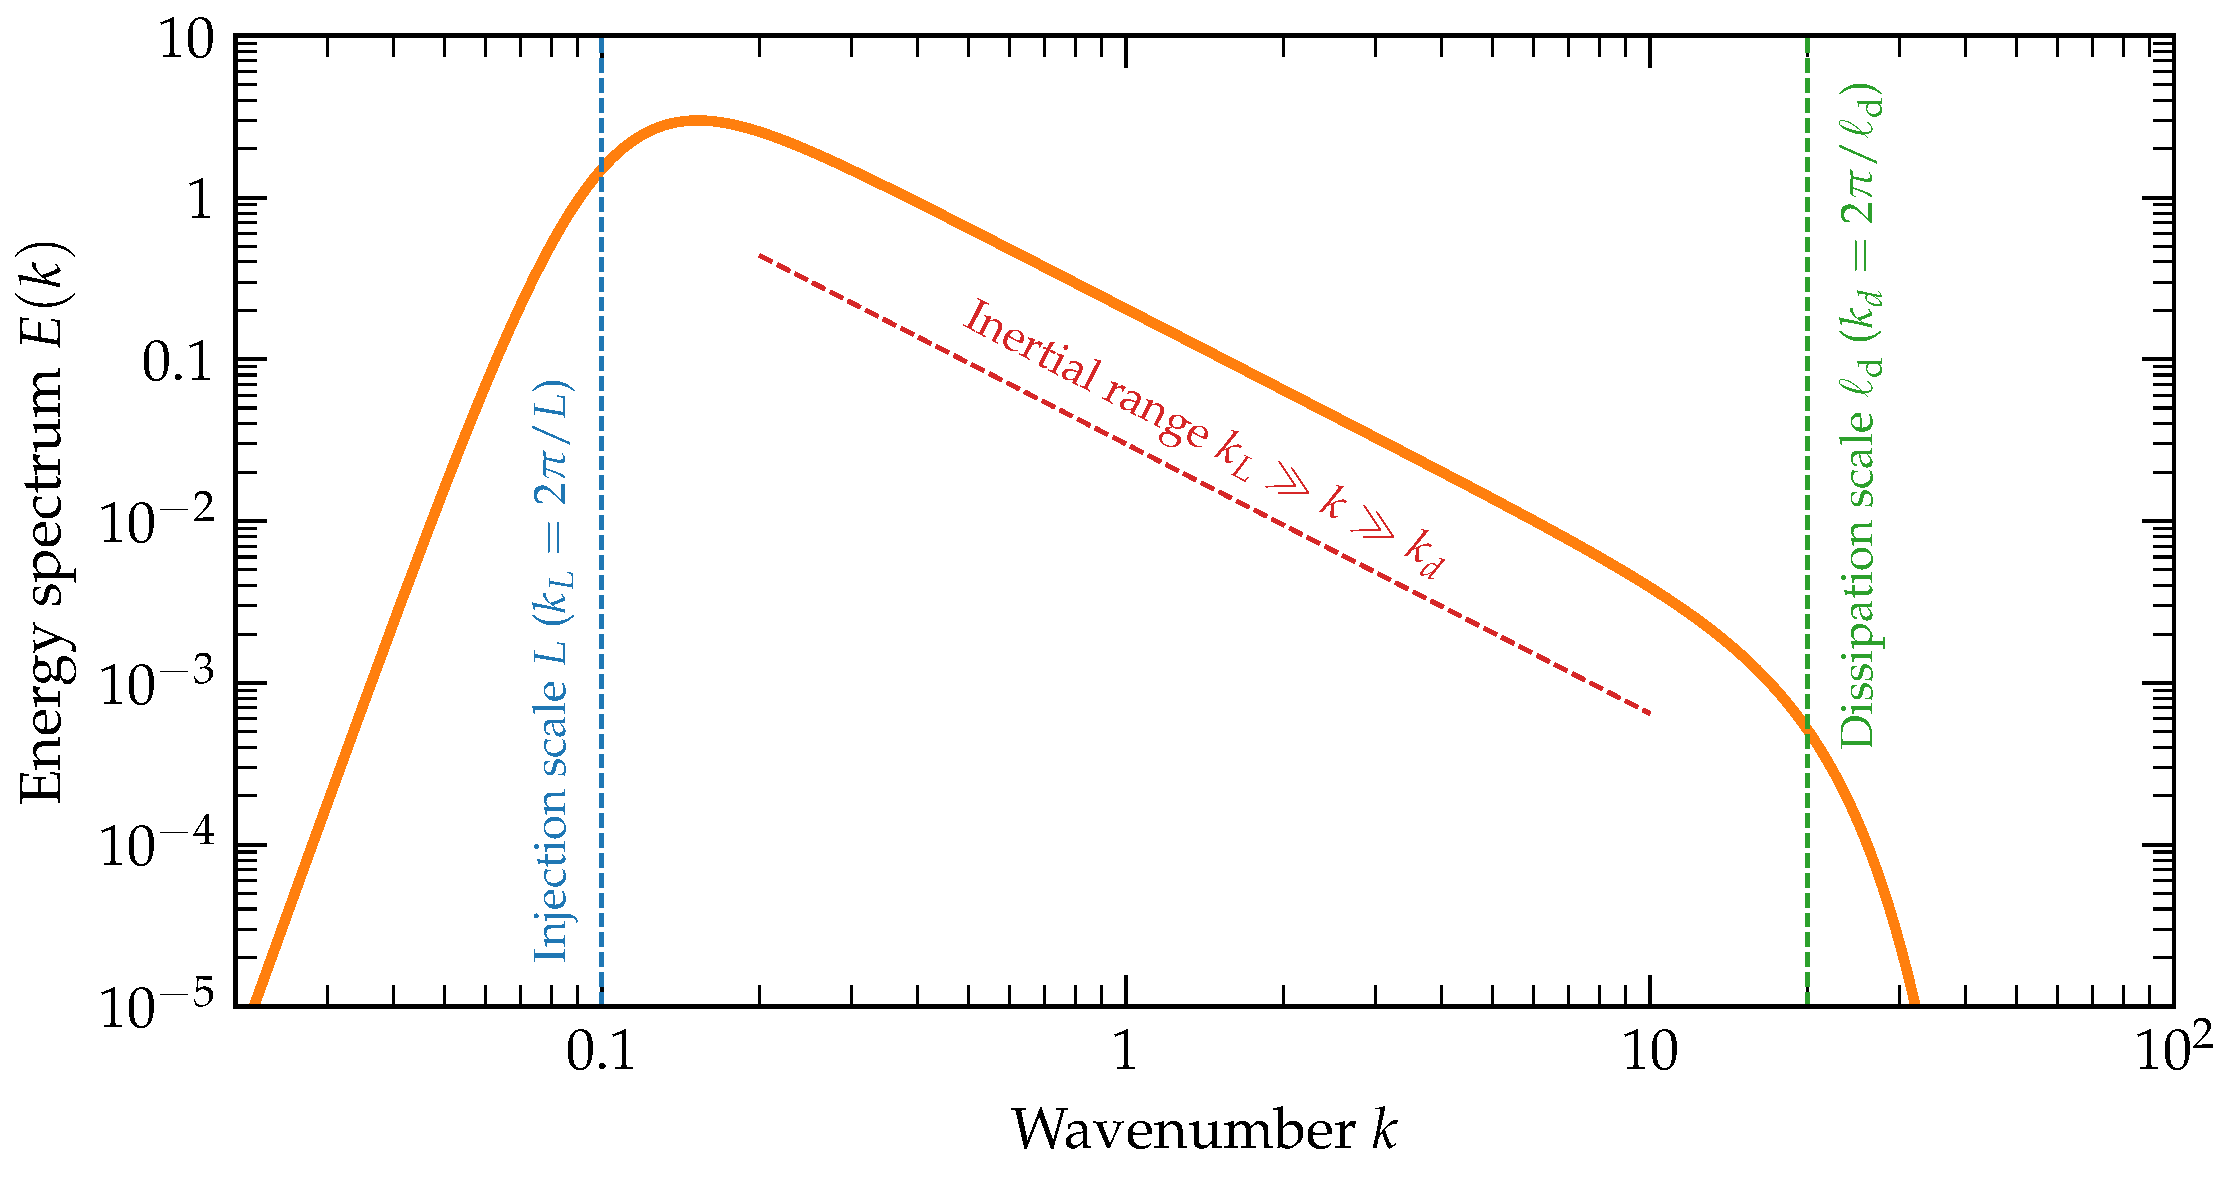
\includegraphics[width=0.99\textwidth]{figures/kolmogorov_cascade_schematic.pdf} 
\caption{.} 
\label{fig:kolmorogov} 
\end{figure}

%Richardson (1922) introduced the energy cascade concept as: “Big whorls have little whorls that feed on their velocity; And little whorls have lesser and so on to viscosity.”

{\color{red}Dire che la turbolenza viene dalle equazione di Navier-Stokes.}

\begin{figure}[t] 
\centering 
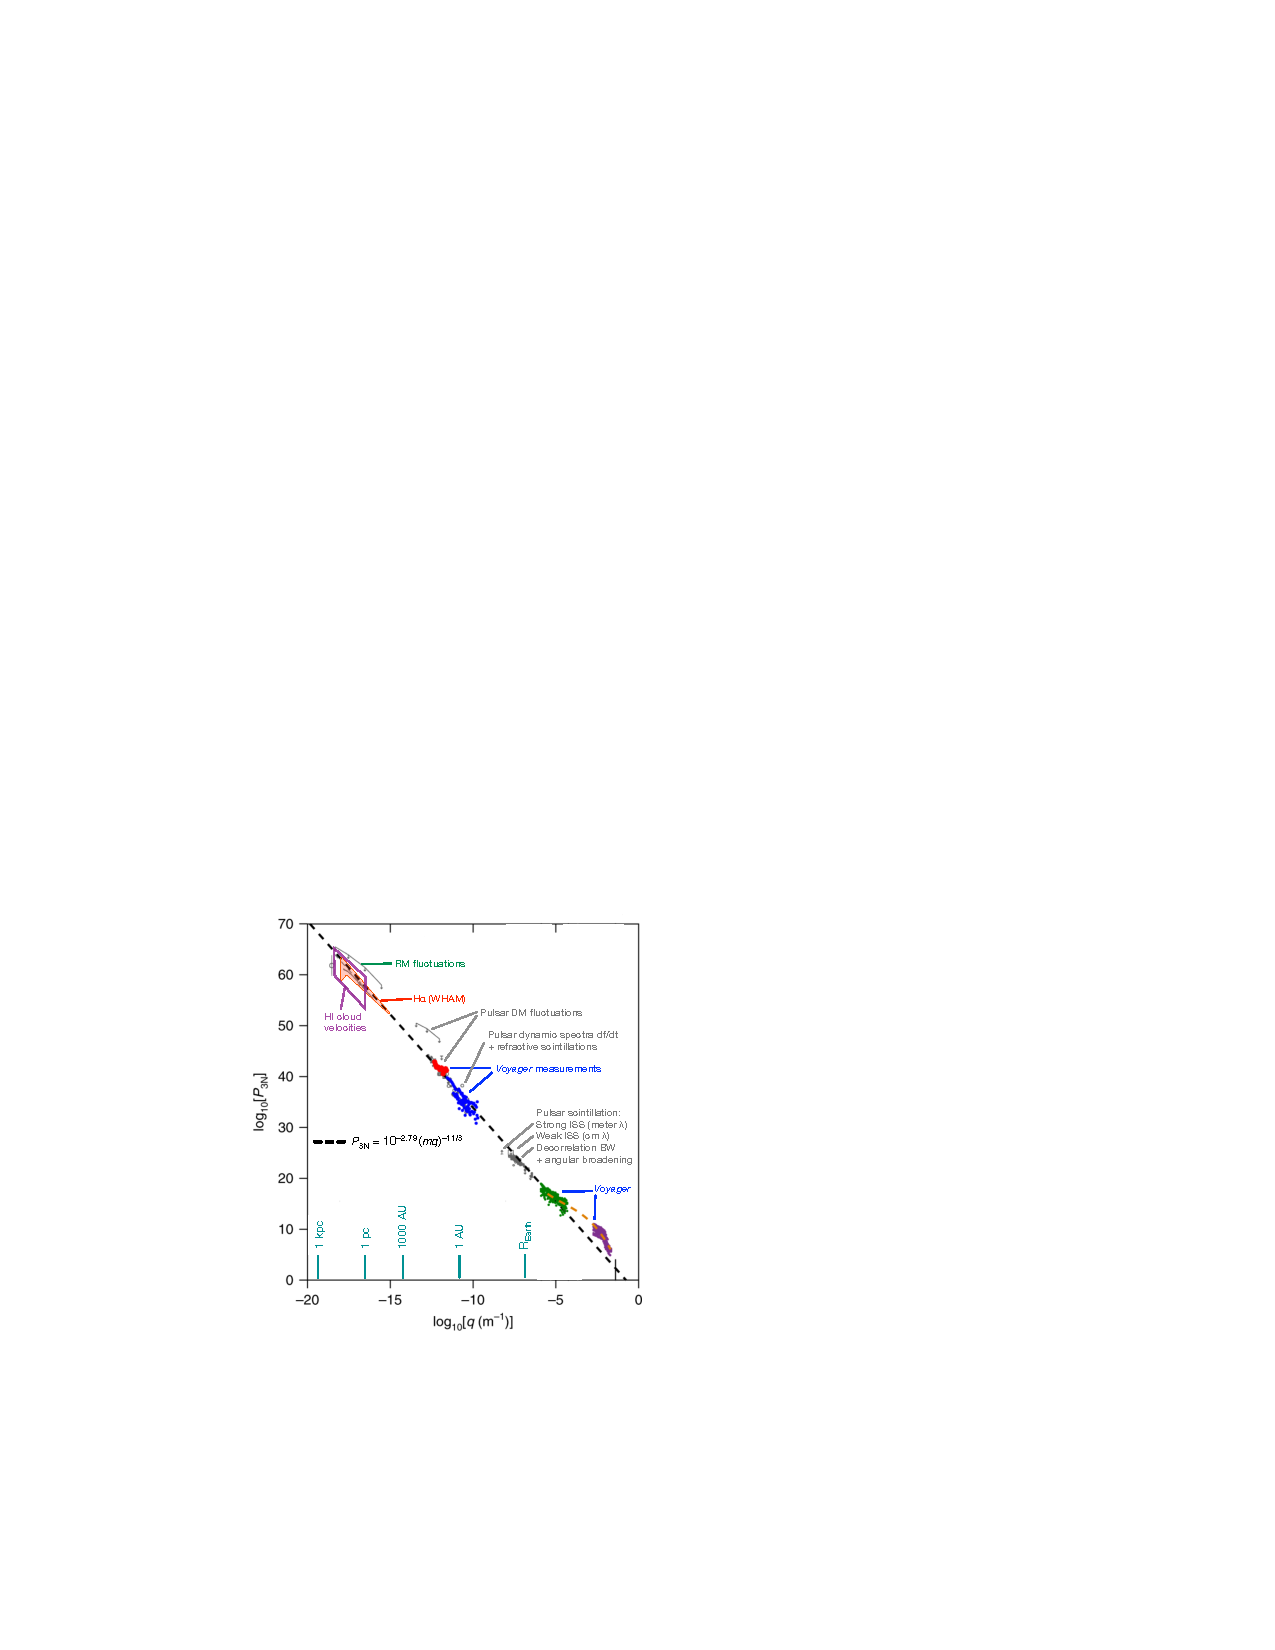
\includegraphics[width=0.7\textwidth]{figures/ism_turbulence.pdf}
\caption{Big Power Law in the sky: electron density power spectrum in the ISM  (Armstrong et al. ApJ 433, 209, 1995) Radio Scintillations measure power
density spectrum in local ISM.. Power law spans 12 decades in
wavenumber space.
Outer
scale
Exhibits a k Kolmogorov-like
spectrum.Power-law in the sky. Armstrong, Nature '81 Spangler '95. ?} 
\label{fig:ismturbulence} 
\end{figure}

\paragraph{From hydrodynamics to MHD: Alfv\'enic cascades.}
In a magnetized plasma the turbulence can be decomposed into Alfvénic and compressive (magnetosonic) parts. The Alfvénic component---incompressible, transverse perturbations tied to the mean magnetic field \(\mathbf B_0\)---dominates much of the ISM cascade. Nonlinear interactions transfer energy mainly by \emph{distorting} counter-propagating Alfvén wave packets. 

Two classic consequences follow:
\begin{itemize}
  \item The cascade is \emph{anisotropic}: eddies become increasingly elongated along \(\mathbf B_0\). In modern language (Goldreich–Sridhar), \emph{critical balance} relates the linear Alfvén time \( (k_\parallel v_A)^{-1} \) to the nonlinear time \( (k_\perp u_{k_\perp})^{-1} \), producing a Kolmogorov-like spectrum \emph{in the perpendicular direction}, \(E(k_\perp)\propto \varepsilon^{2/3}k_\perp^{-5/3}\).
  \item Magnetic and kinetic energies tend toward near-equipartition within the Alfvénic cascade, so the same scaling applies (up to constants) to \(\delta\mathbf v\) and \(\delta\mathbf B\) fluctuations.
\end{itemize}
Older phenomenology (Iroshnikov–Kraichnan) predicts a slightly shallower slope \(k^{-3/2}\) owing to weakened interactions; observations and simulations in many astrophysical settings favor a Kolmogorov-like \(-5/3\) spectrum in \(k_\perp\), with anisotropy set by the mean field strength.

\paragraph{What the inertial range means physically.}
\begin{itemize}
  \item \textbf{Universality:} statistics at \(\ell\) depend only on \(\varepsilon\) (and, in MHD, on the direction relative to \(\mathbf B_0\)), not on how the turbulence was stirred or how it will ultimately dissipate.
  \item \textbf{Self-similar cascade:} energy injected near \(L\) passes through a hierarchy of eddies/wave packets with turnover time \(\tau_\ell\propto \ell^{2/3}\) until it reaches \(\ell_{\rm d}\), where microphysics takes over.
  \item \textbf{Spectral signature:} a power-law energy spectrum—\(E(k)\propto k^{-5/3}\) for hydrodynamic turbulence; in MHD, the same \(-5/3\) scaling appears in the \emph{perpendicular} spectrum of Alfvénic turbulence, with anisotropy \(k_\parallel \ll k_\perp\) that strengthens toward small scales.
\end{itemize}

\paragraph{Takeaway for the Milky Way.}
Large-scale Galactic driving maintains a steady energy flux \(\varepsilon\) into the ISM. In the inertial range, that flux feeds an anisotropic Alfvénic cascade with a Kolmogorov-like perpendicular spectrum. The resulting sea of broadband Alfvénic fluctuations is the natural reservoir of ``where Alfvén waves come from’’ in the Galaxy: they are not produced one frequency at a time, but emerge continuously from the nonlinear cascade that carries energy from \(L\) down to the dissipation scale.

\begin{remark}{Turbulent energy and timescales in the ISM.}

Observations and theory indicate that the Galactic ISM is stirred on large scales by superbubbles and clustered supernovae~\ref{2004Ap&SS.289..323M}. A typical baseline is an outer (forcing) scale \(L\equiv l_0\simeq 100~\mathrm{pc}\) with a characteristic velocity comparable to the sound speed of the warm phases,
\(u_0\sim c_s\simeq 10~\mathrm{km\,s^{-1}}\).

In a Kolmogorov‐type cascade the flow sheds energy at roughly one eddy per scale, so the global decay time of turbulence is set by the turnover time of the largest eddies,
\[
\tau_0 \sim \frac{l_0}{u_0}
\;\simeq\; 10^{7}~\mathrm{yr}.
\]
Thus, even if microscopic dissipation is weak, sustained turbulence requires continuous driving on $\sim$Myr timescales.

The corresponding (mass‐specific) energy flux through scales is
\(\varepsilon \sim u_0^{3}/l_0\),
so the \emph{volumetric} turbulent dissipation rate is
\[
\epsilon_{\rm turb} \sim \rho\,\frac{u_0^{3}}{l_0}.
\]
Adopting a representative warm–ISM density \(n\simeq 1~\mathrm{cm^{-3}}\) and
\(\rho\simeq 1.4\,m_p n \approx 2.3\times10^{-24}~\mathrm{g\,cm^{-3}}\),
one obtains
\[
\epsilon_{\rm turb}\;\approx\; 8\times10^{-27}\ \mathrm{erg\,cm^{-3}\,s^{-1}}.
\]

To compare with the available power from supernovae, distribute the SN mechanical luminosity over the star–forming disc volume
\(V\simeq 2\pi h R_d^2\),
with scale height \(h\simeq 100~\mathrm{pc}\) and radius \(R_d\simeq 10~\mathrm{kpc}\).
Using \(E_{\rm SN}=10^{51}~\mathrm{erg}\) and a Galactic rate
\(\mathcal R_{\rm SN}\simeq 1/50~\mathrm{yr^{-1}}\),
\[
\epsilon_{\rm SN}
=\frac{E_{\rm SN}\,\mathcal R_{\rm SN}}{2\pi h R_d^2}
\;\approx\;
3.4\times10^{-25}\ \mathrm{erg\,cm^{-3}\,s^{-1}}.
\]

Is there enough power to maintain the cascade?
The ratio
\(
\tfrac{\epsilon_{\rm turb}}{\epsilon_{\rm SN}} \approx 0.02
\)
shows that only a \(\sim\!2\text{–}3\%\) coupling of SN mechanical energy into turbulent motions is sufficient—comfortably plausible given other sinks (radiation, cosmic rays, winds). In short, with \(L\sim100\ \mathrm{pc}\) and \(u_0\sim10\ \mathrm{km\,s^{-1}}\), the ISM would decay its turbulence in \(\sim10\) Myr unless it is continuously powered, and ordinary supernova activity can readily supply the needed \(\sim10^{-26} \, \mathrm{erg\,cm^{-3}\,s^{-1}}\).
\end{remark}

\subsection{Self–generated Alfv\'en waves: Kulsrud's argument}

Cosmic rays stream through the ISM at individual speeds $\simeq c$, but with a small \emph{bulk} drift $v_D$ along the mean field $\mathbf B_0$ set by their large–scale pressure gradient. When $v_D$ exceeds the Alfv\'en speed $v_A$, the CR distribution becomes slightly anisotropic in pitch angle and resonantly excites forward–propagating Alfv\'en waves. Those waves then scatter the CRs in pitch angle until, in the frame moving with the waves, the distribution is nearly isotropic. In that process, CRs transfer parallel momentum to the waves/plasma, reducing their bulk drift from $v_D$ down to (approximately) $v_A$. This is Kulsrud's central insight: \emph{streaming CRs self-generate the very Alfv\'en turbulence that limits their own streaming speed.}

\paragraph{Momentum and energy bookkeeping in one line.}
Think of a thin flux tube along $s$.
As CRs are pitch–angle scattered by forward Alfv\'en waves (speed $+v_A$ along $\mathbf B_0$), they become isotropic in the \emph{wave frame}. In the lab frame this means their net parallel momentum density decreases; by momentum conservation, an equal and opposite momentum is given to the waves/plasma. The rate of work done on the waves per unit volume is then
\[
\mathcal{P}_{\rm cr\to w}
\;\simeq\;
(v_D - v_A)\,\bigl|\partial_s P_{\rm cr}\bigr| ,
\]
where $P_{\rm cr}$ is the CR pressure. 
If the wave magnetic energy density is $W\equiv \delta B^2/8\pi$ (cgs),
\[
\frac{{\rm d}W}{{\rm d}t} \;=\; (v_D - v_A)\,\bigl|\partial_s P_{\rm cr}\bigr| 
\quad\Rightarrow\quad 
\text{growth until $v_D\to v_A$ or balanced by damping.}
\]
This captures the physics without yet invoking the resonance details: CRs do work on waves until their bulk motion matches the Alfv\'en frame, at which point no further net momentum can be extracted.

\paragraph{Resonant view and the growth rate $\gamma(k)$.}
The small anisotropy that drives the instability couples to Alfv\'en waves by the gyroresonance condition
\[
\omega - k_\parallel v\mu \;=\; \pm \,\Omega/\gamma,
\qquad \omega \approx k_\parallel v_A,
\]
with $\mu$ the pitch–angle cosine, $\Omega$ the nonrelativistic gyrofrequency, and the upper/lower sign for forward/backward waves.
For $v\!\approx\!c\gg v_A$ the resonant wavenumber mainly selects particles by their gyroradius,
\[
k_{\rm res} \simeq \frac{1}{r_g}=\frac{Ze\,B_0}{pc}.
\]
Linear theory (Kulsrud–Pearce–Skilling) then gives the wave growth rate
\[
\boxed{\;
\gamma(k) \;=\; \frac{\pi}{4}\,\Omega_p\,
\frac{n_{\rm cr}(>p_{\rm res})}{n_i}\,
\Bigl(\frac{v_D}{v_A}-1\Bigr)
\;}
\quad\text{with}\quad
p_{\rm res}=\frac{Ze\,B_0}{k\,c}.
\]
Here $n_{\rm cr}(>p_{\rm res})$ is the number density of CRs with momentum exceeding $p_{\rm res}$, $n_i$ is the ion density, and $\Omega_p=eB_0/(m_pc)$.
The wave energy at wavenumber $k$ obeys
\[
\frac{\partial W(k)}{\partial t} \;=\; 2\,\gamma(k)\,W(k)\;-\;2\,\Gamma_{\rm damp}(k)\,W(k),
\]
so in steady state $\gamma(k)=\Gamma_{\rm damp}(k)$ and the drift adjusts to
\[
\frac{v_D}{v_A}-1\;\simeq\;
\frac{4}{\pi}\,\frac{\Gamma_{\rm damp}(k)}{\Omega_p}\,
\frac{n_i}{n_{\rm cr}(>p_{\rm res})}.
\]
When damping is modest, $v_D\!\to\! v_A$: CRs stream at approximately the Alfv\'en speed.

\paragraph{Connecting the two pictures.}
The resonant formula above explains \emph{which} scales grow (those resonant with CRs of gyroradius $r_g=1/k$) and \emph{how fast}. The global momentum–energy argument explains \emph{why} growth stops: once scattering has isotropized the CRs in the wave frame, the net parallel momentum transfer vanishes and so does the power into waves. Both viewpoints lead to the same physical end–state: a sea of Alfv\'en waves with amplitudes set by the competition between CR driving and damping, and a CR drift regulated to $\simeq v_A$.

\paragraph{What sets the amplitude in the ISM.}
In different phases of the ISM the relevant damping can be ion–neutral friction, non-linear Landau damping, turbulent damping by the ambient cascade, or simple collisional/resistive losses.
Balancing $\gamma(k)$ against the dominant $\Gamma_{\rm damp}(k)$ fixes $\delta B(k)$ (via $W=\delta B^2/8\pi$) and thus the local scattering rate $D_{\mu\mu}(p)$ and parallel diffusion coefficient $\kappa_\parallel(p)$—closing the loop between CR transport and their self-generated turbulence.

\paragraph{Takeaway.}
Super–Alfv\'enic CR streaming is unstable: CRs resonantly excite Alfv\'en waves and, by pitch-angle scattering, hand over enough parallel momentum that their \emph{bulk} speed relaxes from $v_D$ to $\sim v_A$. The energy transferred to the waves grows at a rate set by the CR pressure gradient, while the $k$–by–$k$ growth rate selects scales comparable to CR gyroradii. In this sense, the Galaxy can \emph{manufacture} its own Alfv\'enic turbulence out of the CR pressure it already contains.


\end{document}

%---
%
%## One-line takeaway
%
%Treat a thin flux tube as a string: magnetic tension (T\sim B_0^2 A/4\pi) pulls it taut; inertia is the tube’s linear density (\mu=\rho A); the transverse wave speed is (v_A=\sqrt{T/\mu}=B_0/\sqrt{4\pi\rho}) (or (B_0/\sqrt{\mu_0\rho}) in SI). That’s why your “tension / linear density” rule works for Alfvén waves. 
%
%If you want, I can turn this into a small annotated figure (string vs. flux-tube) to drop straight into the slides.
